\section{The Parameter Analysis for GAN}
\begin{figure*}
	\centering
	\begin{subfigure}{\linewidth}
		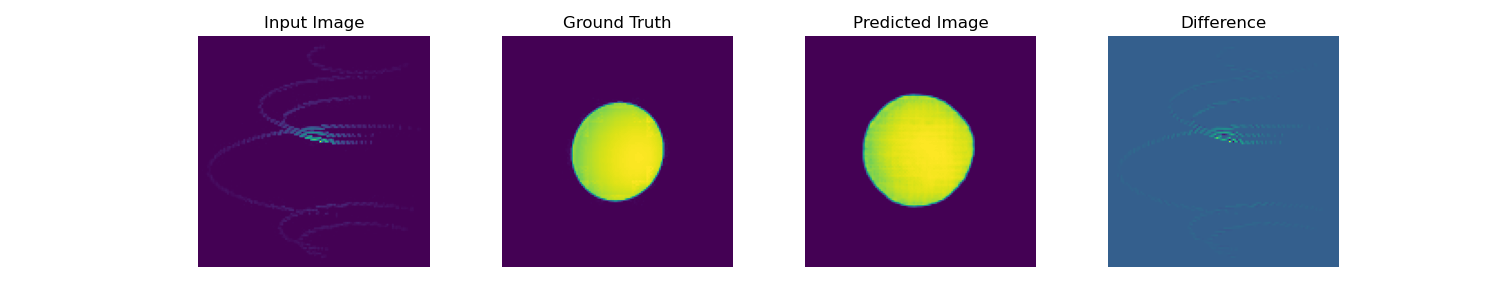
\includegraphics[width=\linewidth]{fig/testing_image/image_0.png}
	\end{subfigure}
	\begin{subfigure}{\linewidth}
		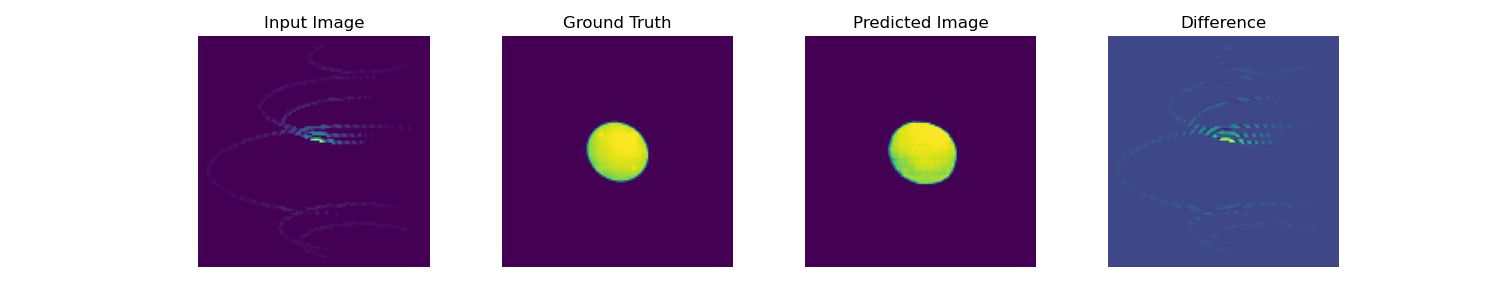
\includegraphics[width=\linewidth]{fig/testing_image/image_16.png}
	\end{subfigure}
	\begin{subfigure}{\linewidth}
		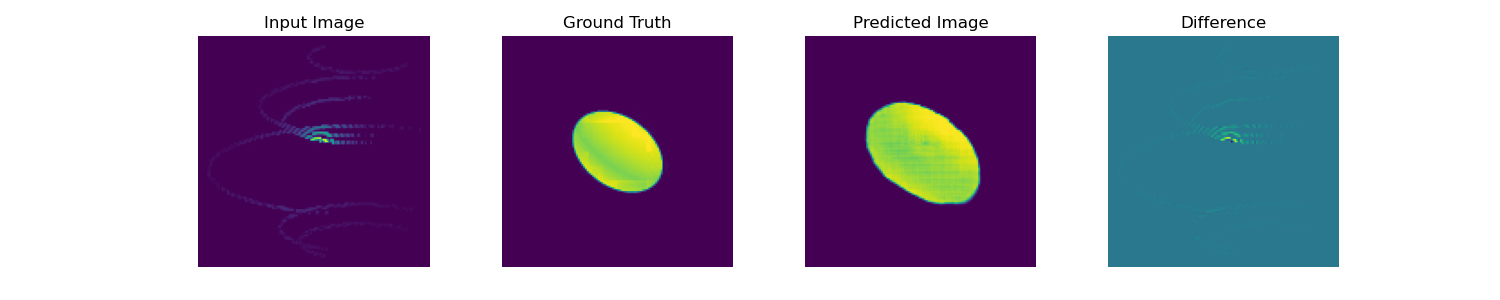
\includegraphics[width=\linewidth]{fig/testing_image/image_35.png}
	\end{subfigure}
	\begin{subfigure}{\linewidth}
		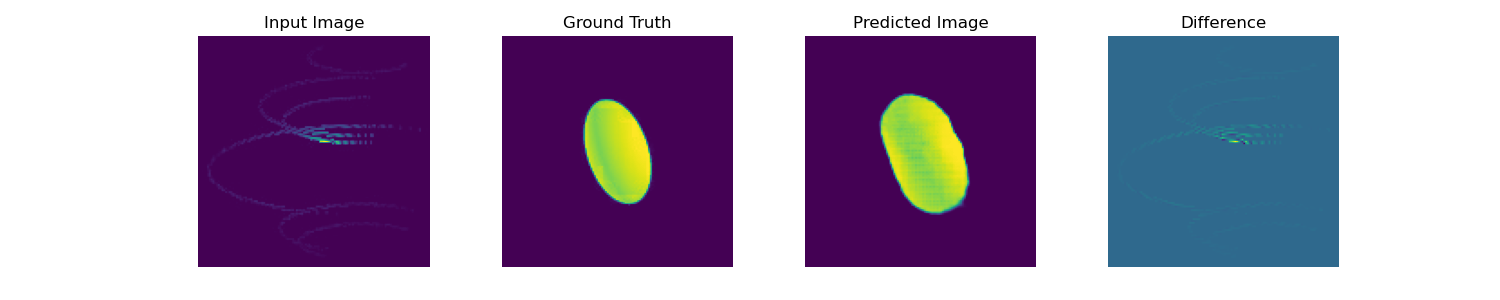
\includegraphics[width=\linewidth]{fig/testing_image/image_38.png}
	\end{subfigure}
	\begin{subfigure}{\linewidth}
		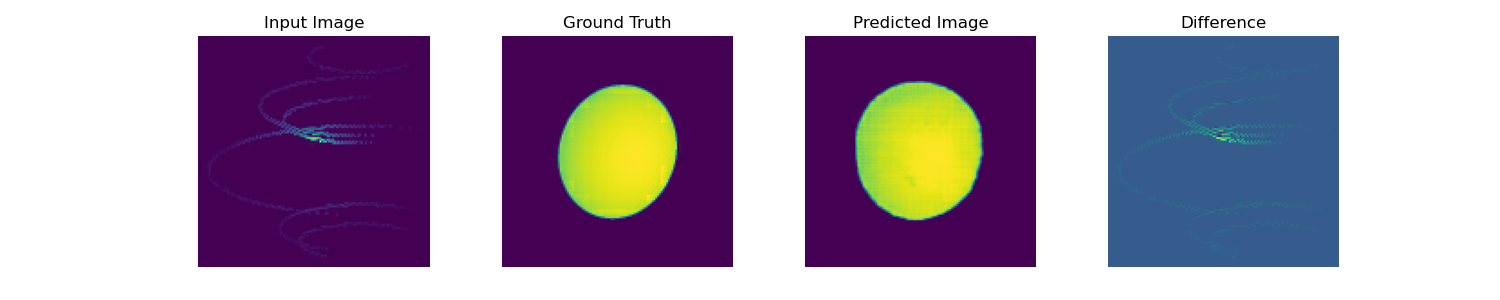
\includegraphics[width=\linewidth]{fig/testing_image/image_42.png}
	\end{subfigure}
	\begin{subfigure}{\linewidth}
		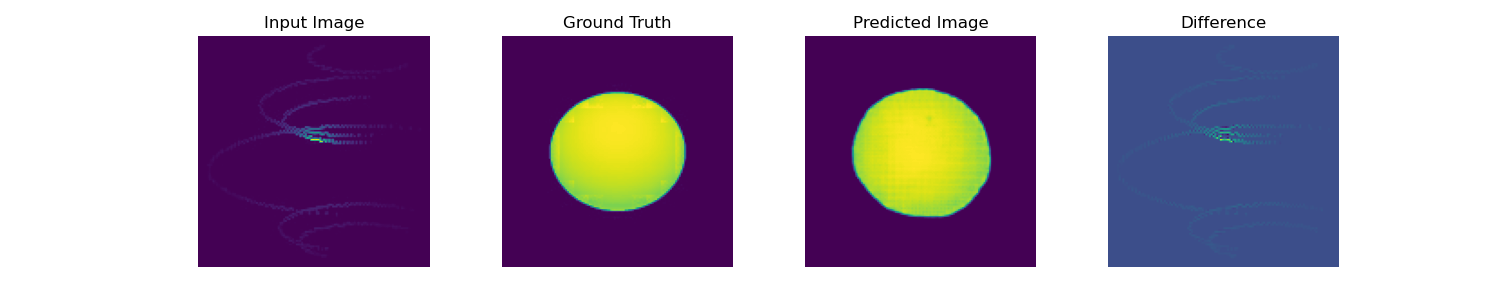
\includegraphics[width=\linewidth]{fig/testing_image/image_47.png}
	\end{subfigure}
	\caption{This set of figures shows the result of GAN for II. The left panels are signals using six baselines, which work as input for GAN. The first middle panel is the real image, also called ground truth, and GAN tries to mimic it during the training. The second middle panel is the reconstructed image, also called the predicted image, with trained GAN, and the end panel is the difference between the ground truth and the predicted image.}
	\label{fig:GAN}
\end{figure*}
Here, we discuss the parameters for the GAN structure, which is trained to reconstruct the image of stellar objects using II. Due to the adversarial nature of GAN, where the generator and discriminator compete in a min-max game, careful tuning of key parameters ensures that both networks are in good term to train the model.

\subsection{Data preparation}
First, we simulate fast-rotating stars, which are modeled as oblate spheroids with different radii and oblateness between 0.5 and 1. Different viewed angles have also been considered, with the effect of gravity darkening being linear dependence. The traced ellipses arise when integrating over the hour angle of the source. For the hyperparameter tuning and comparison of different telescopes, the total hour angle is about 11.5 hours. The ellipses are plotted and converted into grayscale images, resized, and stored as pure arrays to simplify further analysis. 
\begin{figure*}
	\centering
	\begin{subfigure}{0.33\linewidth}
		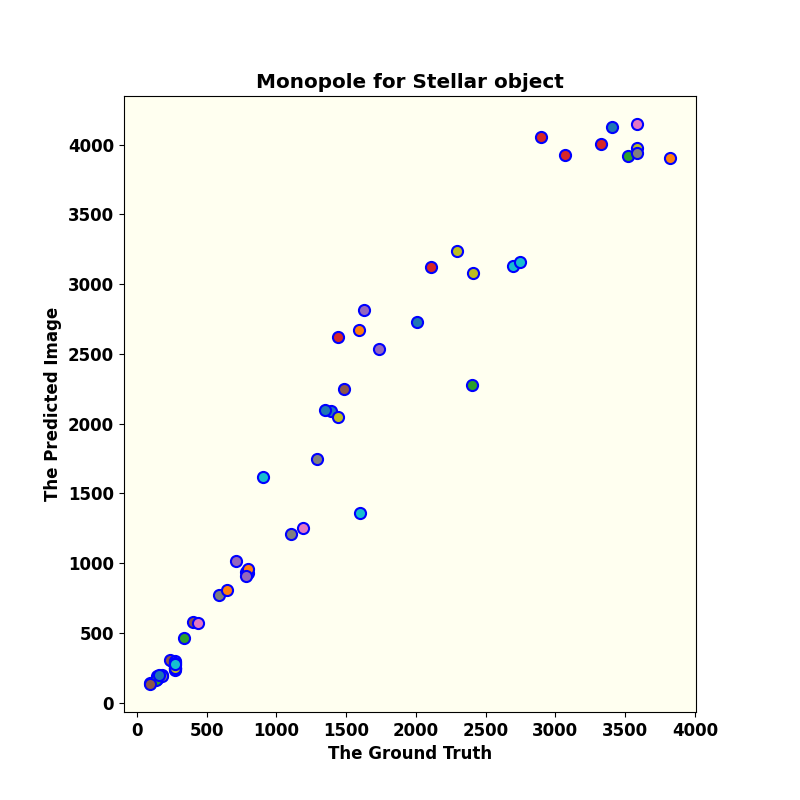
\includegraphics[width=\linewidth]{fig/moments/mom0.png}
		\caption{The monopole.}
		\label{fig:mom1}
	\end{subfigure}\hfill
	\begin{subfigure}{0.33\linewidth}
		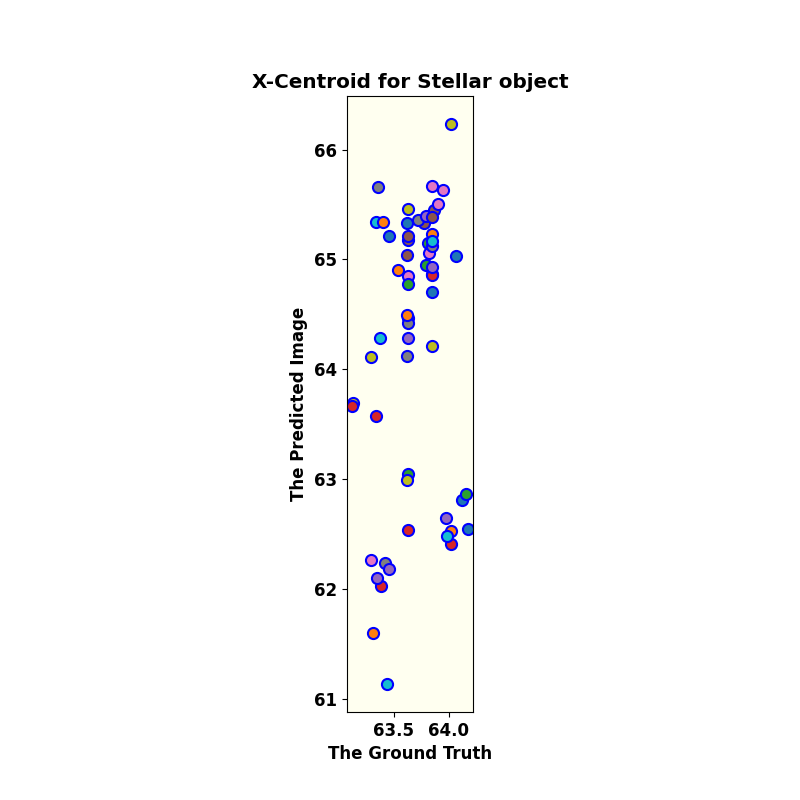
\includegraphics[width=\linewidth]{fig/moments/mom1.png}
		\caption{The centroids along x direction.}
		\label{fig:mom2}
	\end{subfigure}\hfill
	\begin{subfigure}{0.33\linewidth}
		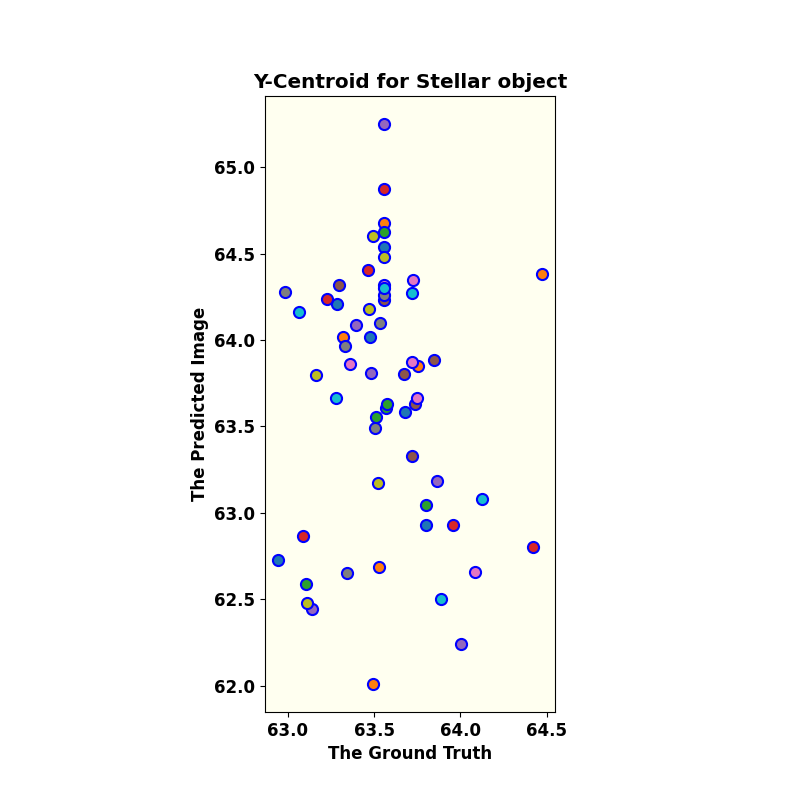
\includegraphics[width=\linewidth]{fig/moments/mom2.png}
		\caption{The centroids along y direction.}
		\label{fig:mom3}
	\end{subfigure}\hfill
	\caption{This set of figures shows the comparison of monopole, x-centroid, and y-centroid for ground truth and predicted images generated by trained GAN.}
	\label{fig:cen}
\end{figure*}
\begin{figure*}
	\centering
	\begin{subfigure}{0.33\linewidth}
		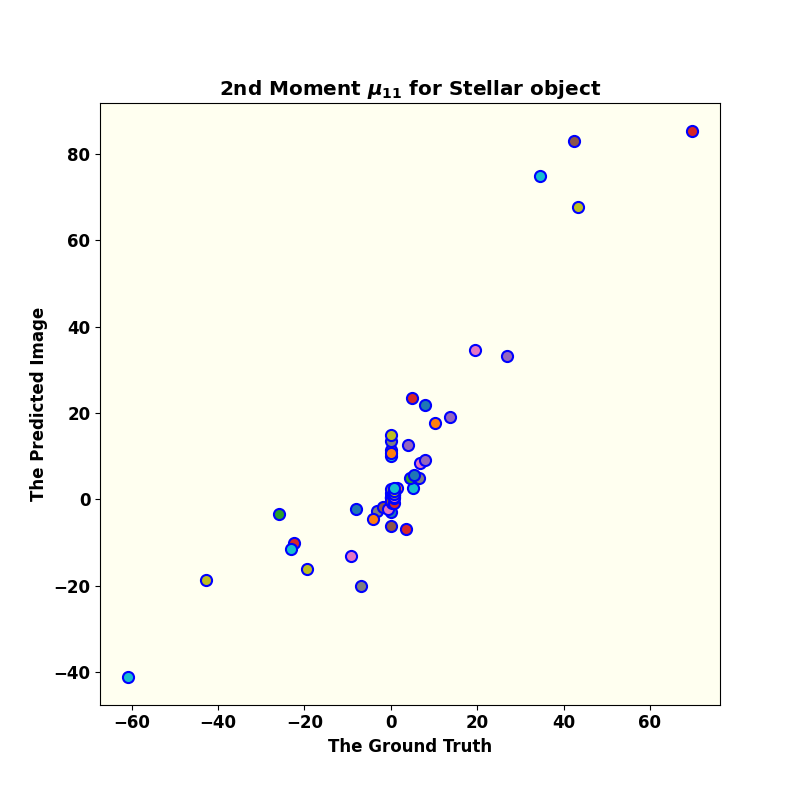
\includegraphics[width=\linewidth]{fig/moments/mom3.png}
		\caption{The 2nd order moment $\mu_{11}$.}
		\label{fig:mom4}
	\end{subfigure}\hfill
	\begin{subfigure}{0.33\linewidth}
		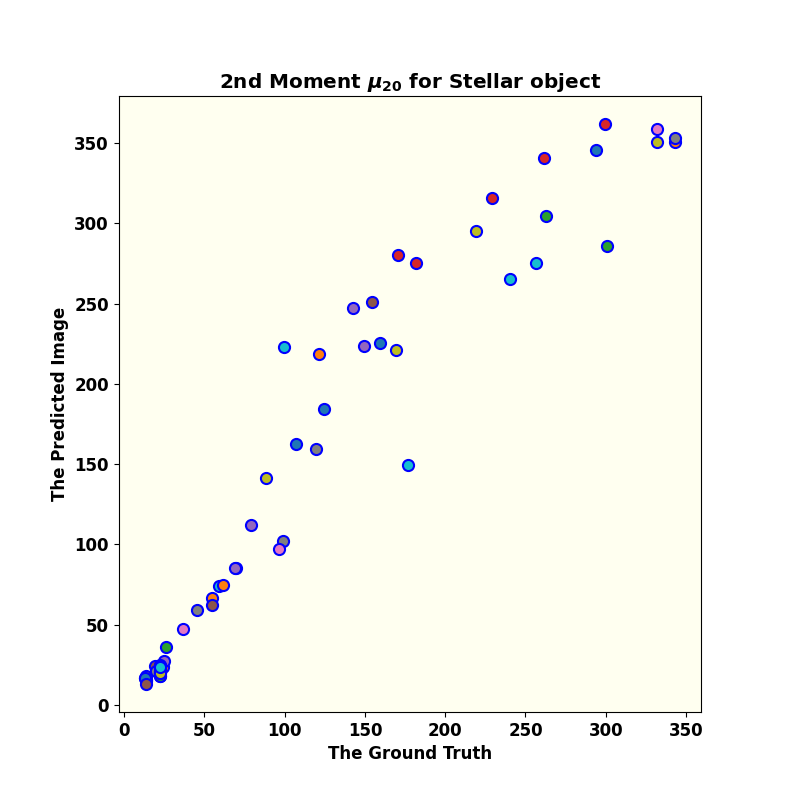
\includegraphics[width=\linewidth]{fig/moments/mom4.png}
		\caption{The 2nd order moment $\mu_{20}$.}
		\label{fig:mom5}
	\end{subfigure}\hfill
	\begin{subfigure}{0.33\linewidth}
		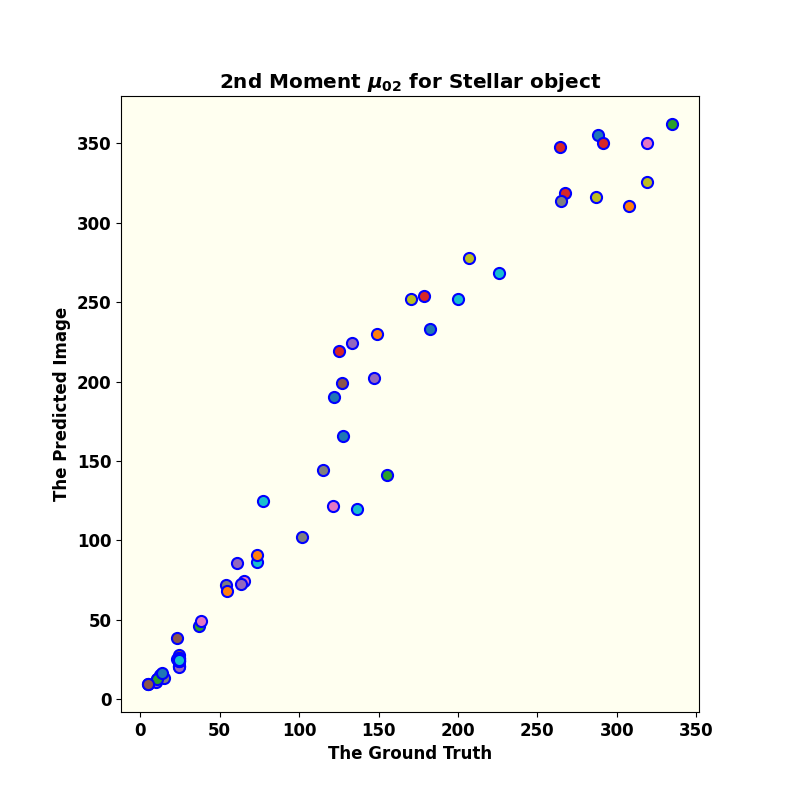
\includegraphics[width=\linewidth]{fig/moments/mom5.png}
		\caption{The 2nd order moment $\mu_{02}$.}
		\label{fig:mom6}
	\end{subfigure}\hfill
	\caption{The second-order central moments provide information about the size and shape of stellar objects. This set of figures shows all the second-order central moments for ground truth and predicted images generated by trained GAN.}
	\label{fig:struc}
\end{figure*}
\begin{figure*}
	\centering
	\begin{subfigure}{0.50\linewidth}
		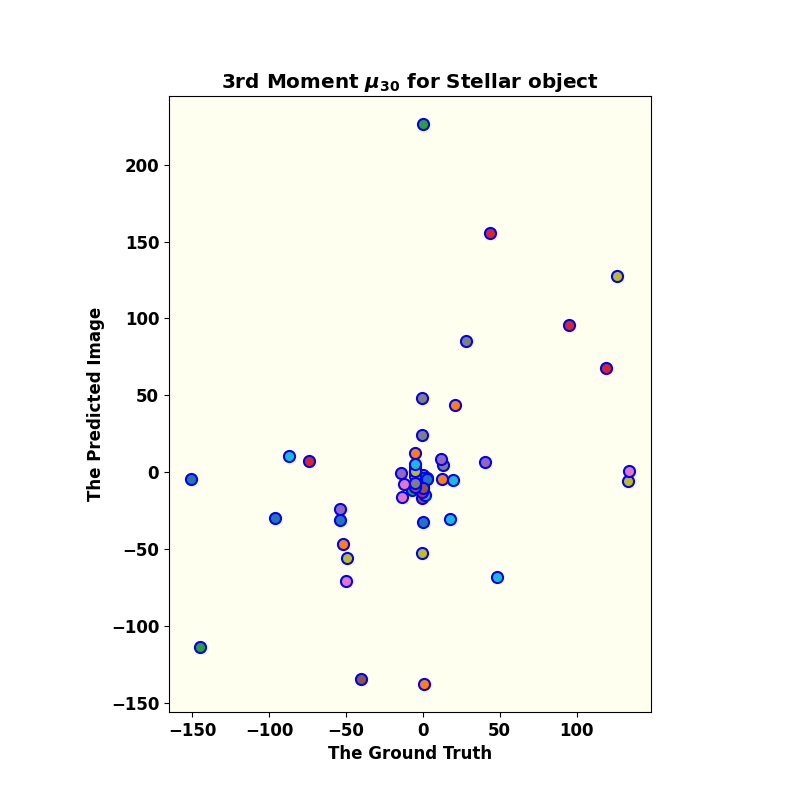
\includegraphics[width=\linewidth]{fig/moments/mom6.png}
		\caption{The 3rd order moment $\mu_{30}$.}
		\label{fig:mom7}
	\end{subfigure}\hfill
	\begin{subfigure}{0.50\linewidth}
		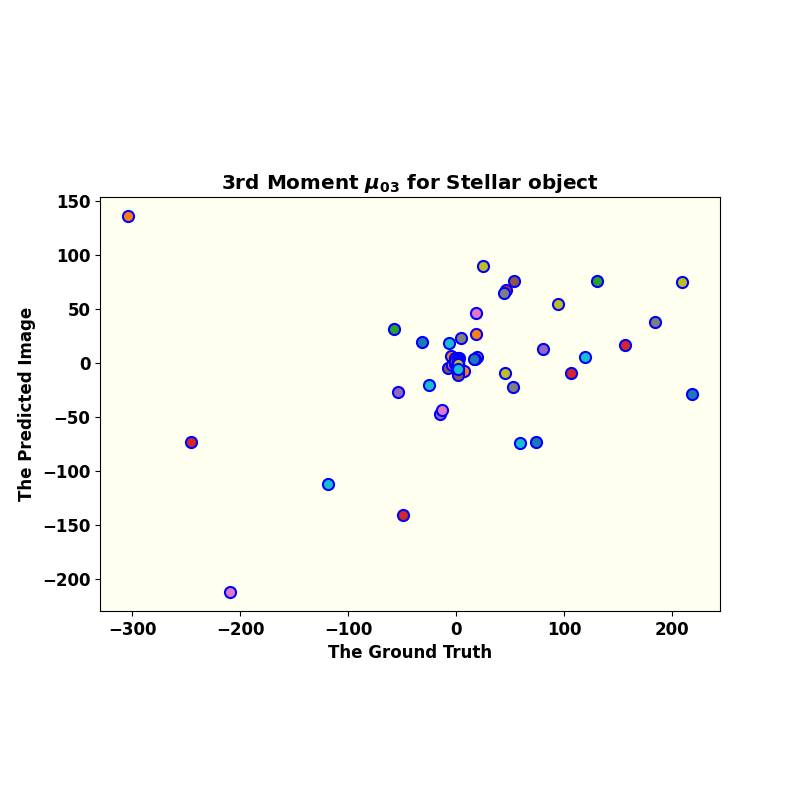
\includegraphics[width=\linewidth]{fig/moments/mom7.png}
		\caption{The 3rd order moment $\mu_{03}$.}
		\label{fig:mom8}
	\end{subfigure}\hfill
	\begin{subfigure}{0.50\linewidth}
		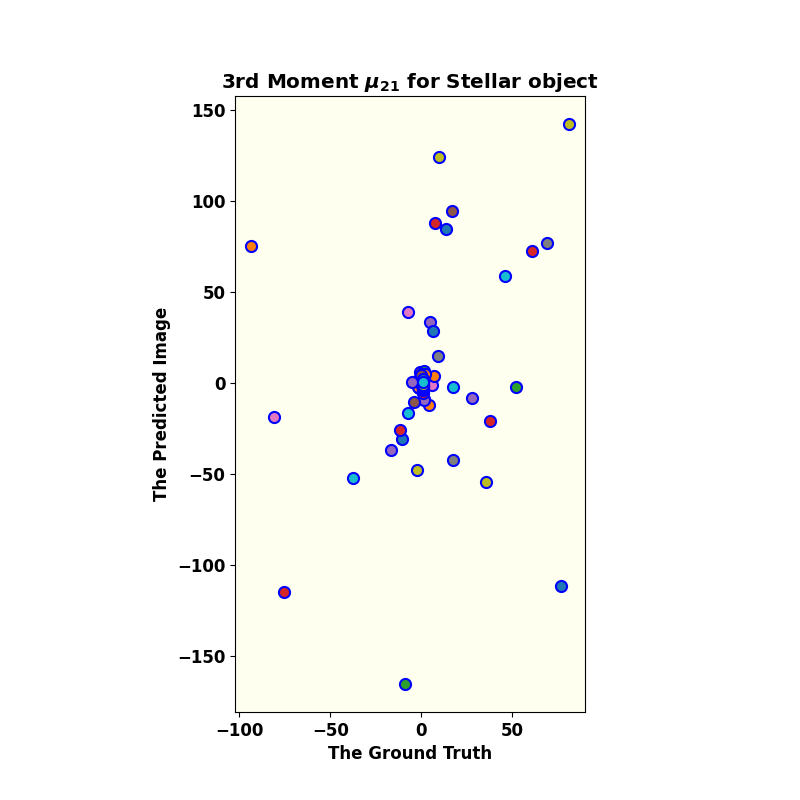
\includegraphics[width=\linewidth]{fig/moments/mom8.png}
		\caption{The 3rd order moment $\mu_{21}$.}
		\label{fig:mom9}
	\end{subfigure}\hfill
	\begin{subfigure}{0.50\linewidth}
		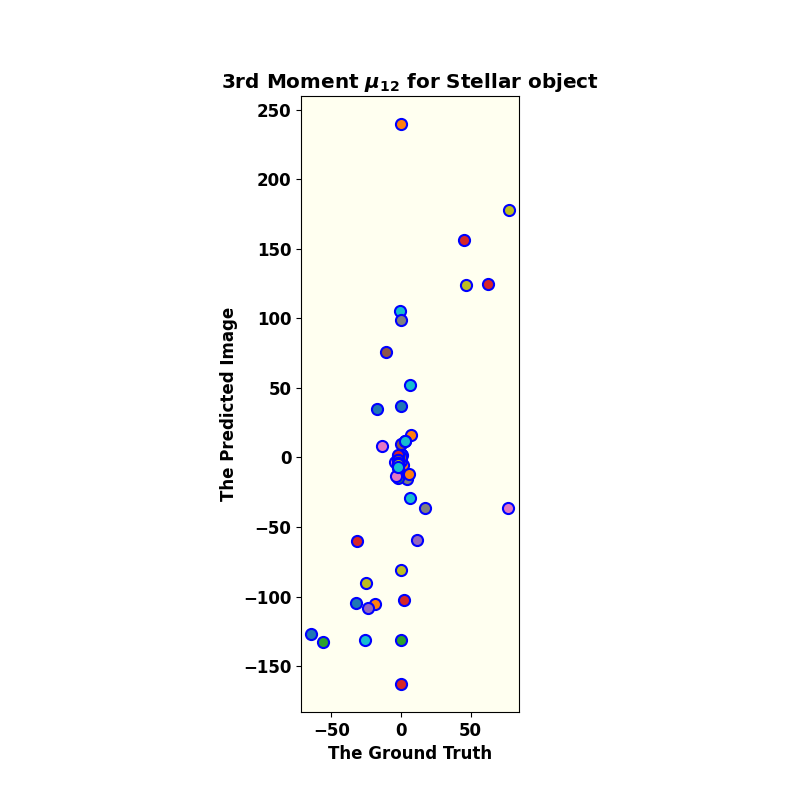
\includegraphics[width=\linewidth]{fig/moments/mom9.png}
		\caption{The 3rd order moment $\mu_{12}$.}
		\label{fig:mom10}
	\end{subfigure}\hfill
	\caption{This set of figures shows all the 3rd-order central moments for ground truth and predicted images generated by trained GAN. It calculates the skewness and evaluates the brightness distribution of images.}
	\label{fig:moments}
\end{figure*}

First, Salt and Pepper noise is introduced at a rate of $\alpha$ (usually 0.5\%). Then, the images are resized, and the mean is subtracted. A two-dimensional Fast Fourier Transform, as well as a Fourier shift, is applied, which yields a complex number of every pixel. As II does not measure the phase, the absolute value is calculated (shown in Fig.~\ref{fig:ft} on a linear and logarithmic scale for visualization). The sparse sampling is also introduced, namely by a pixel-wise multiplication between the absolute valued Fourier transformed image and the sparse sampling map. The result is a map in the Fourier plane with several ellipses, also called the sparse sampling map. Fig.~\ref{fig:ft_base} shows the sparse sampling for Fig.~\ref{fig:image} as the source with four telescopes (Fig.~\ref{fig:teles}). Finally, the pixels are normalized and converted to 8-bit integers. This image represents the sparsely sampled complex visibility, as it can be measured with II. The image shown in Fig.~\ref{fig:ft_base} is the input image for the GAN, which also requires the ground truth image. So, the simulated stars are also resized using the same algorithm and converted to 8-bit integers to reduce the bias. The GAN must know the ground truth corresponding to an input image. Hence, they are merged side-by-side, shown in Fig.~\ref{fig:GANinput}, and used as input to train the GAN. This procedure is conducted for all the simulated stars, with 10\% acting as test data, 10\% as validation data, and the remaining 80\% as training data. 

\subsection{GAN architecture}
The GAN used in this work is based on pix2pix \citep{isola2017image}, which uses a cGAN discussed in the last section. It is very robust and could already be applied to various problems. An example can be found in the TensorFlow tutorials\footnote{\url{https://www.tensorflow.org/tutorials/generative/pix2pix}}, where it is applied to a data set of architectural facades. However, to adapt the pix2pix GAN for the phase retrieval problem, some modifications are necessary. The network uses the TensorFlow \citep{abadi2016tensorflow} library, calculations are performed with scipy \citep{virtanen2020scipy}, and plots are drawn with matplotlib \citep{4160265}.
\begin{figure*}
	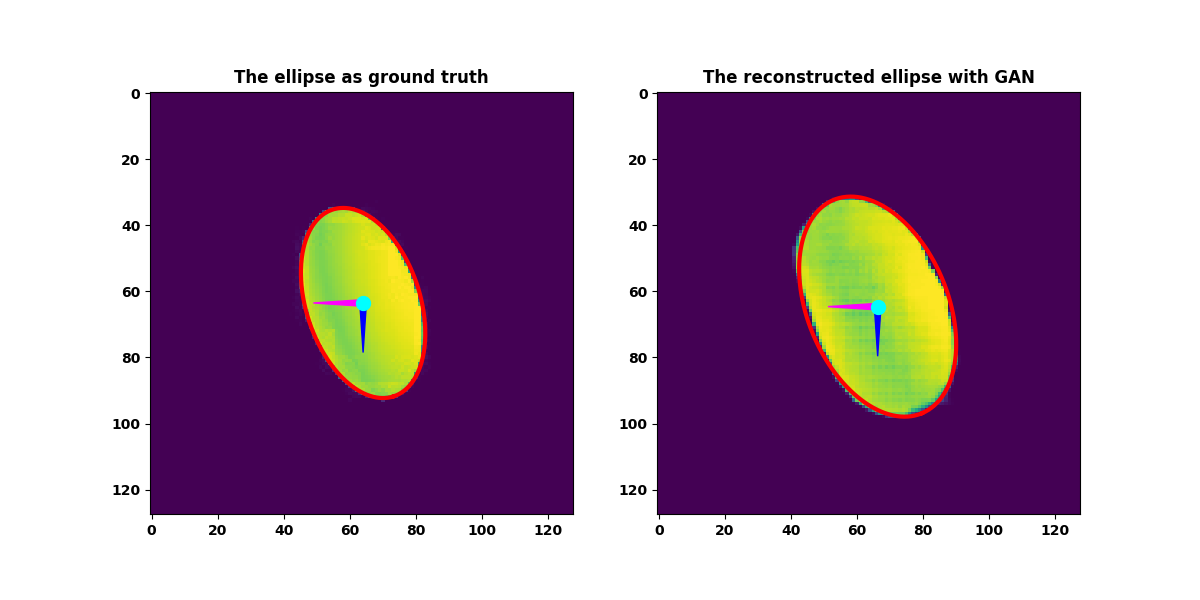
\includegraphics[width=\linewidth]{fig/reconstruction.png}
	\caption{The elliptical image of ground truth and predicted image by trained GAN. The elliptic curve (in red) was drawn using the second-order moment, and cyan dots show the centroids (mx, my) of the images. There are two arrows in each image showing the skewness of pixel distribution along the x and y axes (magenta and blue color).}
	\label{fig:recons}
\end{figure*}
\subsection{Hyperparameter tuning}
The GAN used for this work depends on several parameters, which will be explained here briefly (an in-depth discussion can be found in \citep{murphy2022probabilistic}).

The learning rate of the optimizer is a measure of how much the model changes per iteration. Small learning rates can lead to underfitting, and large learning rates can make the model unstable. It is therefore important to carefully choose the learning rate \citep{murphy2022probabilistic}. Fig.~\ref{fig:Plot_learning_rate_loss} shows the effect of the learning rate on both generator and discriminator loss for three different values of it. Both loss functions have fewer outliers with decreasing learning rates, which is expected, as there is less change in the models with low learning rates. Even though all models stabilize at the same level, low learning rates are preferred.

The kernel size is the size of the kernel in the convolutional layer. It determines the amount of pixels that are linearly combined into a new pixel. A large kernel size allows one to catch features that are a few pixels away, but it also means that unrelated features might be introduced. The kernel size does not have a big effect on the loss functions, as shown in Fig.~\ref{fig:Plot_kernel_size_loss}. Smaller kernel sizes seem to have more outliers, which means that either generator or discriminator gains an advantage. Therefore, a kernel size of 5 is preferred.

The amount of noise is reflected by the two parameters $\alpha$ and $\beta$. Both indicate the percentage of pixels that change to either black or white, hence the name Salt and Pepper noise, where $\alpha$ is introduced in the real image, $\beta$ in the generated image. Different ratios $\frac{\alpha}{\beta}$ can lead to different model performances. There is no significant difference between distinct noise rates introduced in the images. Fig.~\ref{fig:Plot_noise_loss} shows the loss functions on smaller images (64 x 64). As there is no effect, it was not necessary to repeat this analysis for larger images. 

The batch size defines the number of images that pass the network simultaneously. It is observed that smaller batch sizes can lead to better generalization \citep{prince2023understanding}. Fig.~\ref{fig:Plot_batchsize_loss} shows two different batch sizes. Here, when two images are processed simultaneously, there are fewer outliers, but since it increases the training time heavily, a batch size of 1 is used.

While training GAN, one can give the discriminator an advantage by increasing the number of training steps before returning to the generator training. It can increase the performance of the model. However, it increases the training time as well and leads to a lower discriminator loss score, as shown in Fig.~\ref{fig:Plot_discrep_loss}. At the same time, the generator score increases slightly, which should be no surprise. Because the generated images did not improve with higher discriminator training, they are usually trained in the same amount as the generator.

Finally, the amount of sparse sampling can be varied, giving the model access to more pixels. More telescopes automatically lead to more baselines and, hence, more pixels that are available. Fig.~\ref{fig:Plot_telescopes_loss} shows the loss functions for different numbers of telescopes. There is a huge disparity, which can partly be explained by the fact that the relation between telescopes and baselines is not linear. The Fourier plane can be sampled sixfold when using four telescopes in contrast to only two telescopes. In the latter case, both the generator and discriminator are not trained smoothly, as seen by the outliers. It is already better with three telescopes and very promising when using four telescopes. The degree of sparse sampling seems to have the biggest effect of all hyperparameters.